% =====================================================================
% 3. Area 1: core architectures
%    Dense (T9) and CNN (T10): own blocks, in depth.
%    RNN (T11) and Transformer (T12): Maria's blocks, summarised and attributed.
% =====================================================================
\section{Area 1: core architectures}\label{sec:arch}

Five families were trained on the same 12-lead input with the protocol of
Section~\ref{sec:framework}. Each block changed one factor at a time against a baseline, with three
seeds per configuration. The dense network and the CNN are my blocks and are analysed in depth; the
recurrent networks and the Transformer are Mar\'ia's blocks and are summarised.

% ---------------------------------------------------------------------
\subsection{Dense network (own block)}\label{sec:dense}

\paragraph{Model and theory.} The record is flattened into a vector of 12\,000 numbers and passed
through two hidden layers of 256 units (Linear $\to$ batch norm $\to$ ReLU $\to$ dropout) and a Linear
layer with five logits (\denseParamsBase{} parameters, almost all of them in the first layer). Each
unit of the first layer computes one weighted sum of the whole record: it has one weight for every
lead and every instant. A QRS complex that occurs 0.3\,s later in another record meets different
weights, so the network has to learn the same shape separately at every position. Nothing in the
architecture says that the input is a time series; this is the limitation that the following
families remove.

Two regularisers are part of the baseline. \emph{Dropout} switches off each hidden unit at random
during training, so every batch trains a different thinned network and no unit can rely on specific
others; at test time all units are used. The rate 0.5 follows Srivastava et al., for whom the retention
probability ``can simply be set at 0.5, which seems to be close to optimal for a wide range of networks
and tasks'' \cite[p.~1930]{srivastava2014dropout}. \emph{Batch normalisation} standardises each
pre-activation with the mean and variance of the current batch and then rescales it with two learned
parameters; it is placed, as in Ioffe and Szegedy, ``immediately before the nonlinearity''
\cite[p.~5]{ioffe2015batch}. At evaluation time it uses running averages collected during training,
so a prediction does not depend on the other records of the batch.

\paragraph{Results.} Table~\ref{tab:dense_ablations} and Figure~\ref{fig:dense_curves} summarise the
ablations.

% Shared float (common/make_floats.py). Table: tables/dense_ablations.tex
\begin{table}[htbp]
\centering
\caption[Dense network: ablations (validation)]{Dense ablations on the validation fold: mean $\pm$ SD over seeds 42--44; $\Delta$ = mean paired difference with the baseline of the same seed; seeds better / worse = seeds whose paired 95\,\% patient-bootstrap interval lies wholly above / below 0.}
\label{tab:dense_ablations}
\small
\begin{adjustbox}{max width=\textwidth}
% Generated by src/dense_experiments.py from results/logs/dense_summary.json.
% Needs report/numbers.tex (alias "dense" in report/runs.json) and \usepackage{booktabs}.
\begin{tabular}{llrcrc}
\toprule
Factor & Configuration & Parameters & Val.\ macro AUROC & $\Delta$ vs.\ baseline & Seeds better / worse \\
\midrule
baseline & Baseline: z-score, BN, dropout 0.5, 2 $\times$ 256 & \denseParamsBase{} & \denseValAurocMeanBase{} $\pm$ \denseValAurocSdBase{} & --- & --- \\
\addlinespace
input scaling & No input z-score (raw mV) & \denseParamsNoNorm{} & \denseValAurocMeanNoNorm{} $\pm$ \denseValAurocSdNoNorm{} & \denseDiffMeanNoNorm{} & \denseNSeedsBetterNoNorm{} / \denseNSeedsWorseNoNorm{} of \denseNSeedsComparedNoNorm{} \\
\addlinespace
batch norm & No batch norm & \denseParamsNoBn{} & \denseValAurocMeanNoBn{} $\pm$ \denseValAurocSdNoBn{} & \denseDiffMeanNoBn{} & \denseNSeedsBetterNoBn{} / \denseNSeedsWorseNoBn{} of \denseNSeedsComparedNoBn{} \\
\addlinespace
input scaling $\times$ batch norm & No input z-score and no batch norm & \denseParamsNoNormNoBn{} & \denseValAurocMeanNoNormNoBn{} $\pm$ \denseValAurocSdNoNormNoBn{} & \denseDiffMeanNoNormNoBn{} & \denseNSeedsBetterNoNormNoBn{} / \denseNSeedsWorseNoNormNoBn{} of \denseNSeedsComparedNoNormNoBn{} \\
\addlinespace
dropout & No dropout & \denseParamsNoDropout{} & \denseValAurocMeanNoDropout{} $\pm$ \denseValAurocSdNoDropout{} & \denseDiffMeanNoDropout{} & \denseNSeedsBetterNoDropout{} / \denseNSeedsWorseNoDropout{} of \denseNSeedsComparedNoDropout{} \\
dropout & Dropout 0.2 & \denseParamsDropoutZeroTwo{} & \denseValAurocMeanDropoutZeroTwo{} $\pm$ \denseValAurocSdDropoutZeroTwo{} & \denseDiffMeanDropoutZeroTwo{} & \denseNSeedsBetterDropoutZeroTwo{} / \denseNSeedsWorseDropoutZeroTwo{} of \denseNSeedsComparedDropoutZeroTwo{} \\
\addlinespace
depth & 1 hidden layer (256) & \denseParamsDepthOne{} & \denseValAurocMeanDepthOne{} $\pm$ \denseValAurocSdDepthOne{} & \denseDiffMeanDepthOne{} & \denseNSeedsBetterDepthOne{} / \denseNSeedsWorseDepthOne{} of \denseNSeedsComparedDepthOne{} \\
depth & 3 hidden layers (256) & \denseParamsDepthThree{} & \denseValAurocMeanDepthThree{} $\pm$ \denseValAurocSdDepthThree{} & \denseDiffMeanDepthThree{} & \denseNSeedsBetterDepthThree{} / \denseNSeedsWorseDepthThree{} of \denseNSeedsComparedDepthThree{} \\
depth & 4 hidden layers (256) & \denseParamsDepthFour{} & \denseValAurocMeanDepthFour{} $\pm$ \denseValAurocSdDepthFour{} & \denseDiffMeanDepthFour{} & \denseNSeedsBetterDepthFour{} / \denseNSeedsWorseDepthFour{} of \denseNSeedsComparedDepthFour{} \\
\addlinespace
width & Width 64 (2 layers) & \denseParamsWidthSixFour{} & \denseValAurocMeanWidthSixFour{} $\pm$ \denseValAurocSdWidthSixFour{} & \denseDiffMeanWidthSixFour{} & \denseNSeedsBetterWidthSixFour{} / \denseNSeedsWorseWidthSixFour{} of \denseNSeedsComparedWidthSixFour{} \\
width & Width 1024 (2 layers) & \denseParamsWidthOneZeroTwoFour{} & \denseValAurocMeanWidthOneZeroTwoFour{} $\pm$ \denseValAurocSdWidthOneZeroTwoFour{} & \denseDiffMeanWidthOneZeroTwoFour{} & \denseNSeedsBetterWidthOneZeroTwoFour{} / \denseNSeedsWorseWidthOneZeroTwoFour{} of \denseNSeedsComparedWidthOneZeroTwoFour{} \\
\bottomrule
\end{tabular}

\end{adjustbox}
\end{table}

% Shared float (common/make_floats.py). Figure: figures/dense_curves.pdf
\begin{figure}[htbp]
\centering
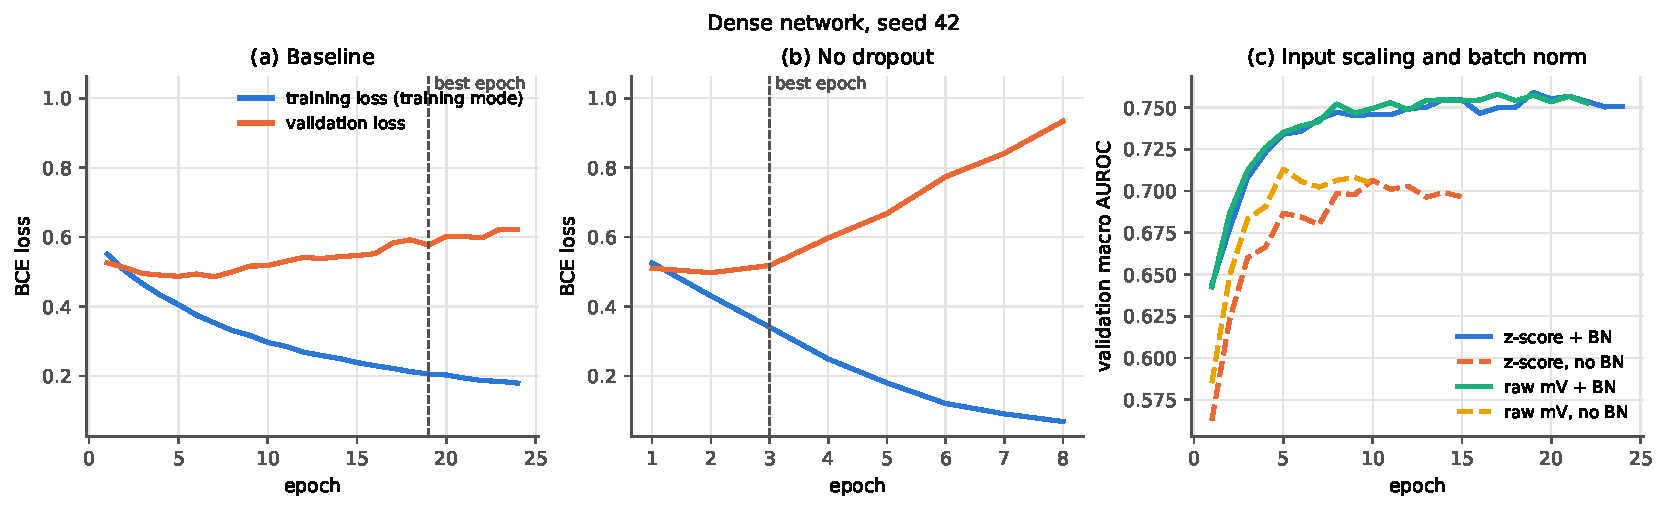
\includegraphics[width=\textwidth,height=0.42\textheight,keepaspectratio]{figures/dense_curves.pdf}
\caption[Dense network: learning curves]{Dense network, seed 42. (a) Baseline: training loss (measured in training mode, with dropout) and validation loss; dashed line: best epoch by validation macro AUROC. (b) The same without dropout. (c) Validation macro AUROC with and without input z-score and batch norm.}
\label{fig:dense_curves}
\end{figure}


\begin{enumerate}[leftmargin=1.4em,itemsep=2pt]
  \item \textbf{Dropout is the main defence against overfitting.} Without it the best epoch is, on
        average, epoch \intval{\denseBestEpochMeanNoDropout}: the training loss keeps falling while the
        validation loss rises (Figure~\ref{fig:dense_curves}b), and the validation AUROC drops by
        \denseDiffMeanNoDropout{} in all seeds. A rate of 0.2 is in between
        (\denseDiffMeanDropoutZeroTwo{}). With \denseParamsBase{} parameters and \edaNLabelledTrain{} training records, the network can
        memorise the training set.
  \item \textbf{Batch norm is essential and absorbs the input scaling.} Removing it costs
        \denseDiffMeanNoBn{} in all seeds. With batch norm, feeding raw millivolts instead of the
        z-scored input changes nothing (\denseDiffMeanNoNorm{}, no seed significant), because the
        first batch-norm layer re-standardises the pre-activations whatever the scale of the input.
        Without batch norm the input scale matters, and unexpectedly the raw millivolts did better
        than the z-score (\denseDiffMeanNoNormNoBn{} against \denseDiffMeanNoBn{}). My explanation, not
        tested: the ECG in millivolts is already on a small scale (training standard deviations between
        \edaLeadStdAVR{} and \edaLeadStdVTwo{}\,mV per lead), so the z-score enlarges the input and
        the first-layer pre-activations several times.
  \item \textbf{Depth and width.} One hidden layer is clearly worse (\denseDiffMeanDepthOne{}); two
        and three are equivalent, four slightly worse. Sixty-four units are too few
        (\denseDiffMeanWidthSixFour{}); 1024 units add nothing and take \denseEpochTimeMeanWidthOneZeroTwoFour{}\,s per epoch against
        \denseEpochTimeMeanBase{}\,s.
        Extra layers change little because the first layer already holds almost every parameter.
  \item \textbf{Validation loss and AUROC disagree} (Figure~\ref{fig:dense_curves}a): the validation
        loss reaches its minimum early and then rises, while the AUROC keeps improving for several
        more epochs. The network keeps ranking the records better while its probabilities become
        over-confident. Early stopping on the AUROC therefore stops later than a rule based on the
        loss would.
  \item \textbf{Only a little better than the trivial model.} The final Dense model reaches a test
        macro AUROC of \denseFinalTestMacroAurocMean{} against \trivialTestMacroAuroc{} for a logistic
        regression on the mean and standard deviation of each lead; the paired difference
        (\denseDiffTrivialMean{} on average) excludes 0 in all seeds, but for MI and CD the point
        estimates are below the trivial model's (Table~\ref{tab:comparison_per_class}; no per-class
        paired test, so this is an observation only).
\end{enumerate}

\paragraph{What the first layer learnt.} The weights of the three most important hidden units look
like noise along time, with no heartbeat template (Figure~\ref{fig:dense_first_layer}), but some
instants show vertical bands in which several limb leads take related or opposite signs. The
augmented limb leads are computed from the same limb electrodes \cite[p.~e263]{wagner2009aha}, so
reading these bands as the network weighing related leads together is plausible, but it remains a
hypothesis. What the figure shows without interpretation is the point of item~5: one weight per
instant, nothing that repeats from beat to beat.

% Shared float (common/make_floats.py). Figure: figures/dense_first_layer.pdf
\begin{figure}[htbp]
\centering
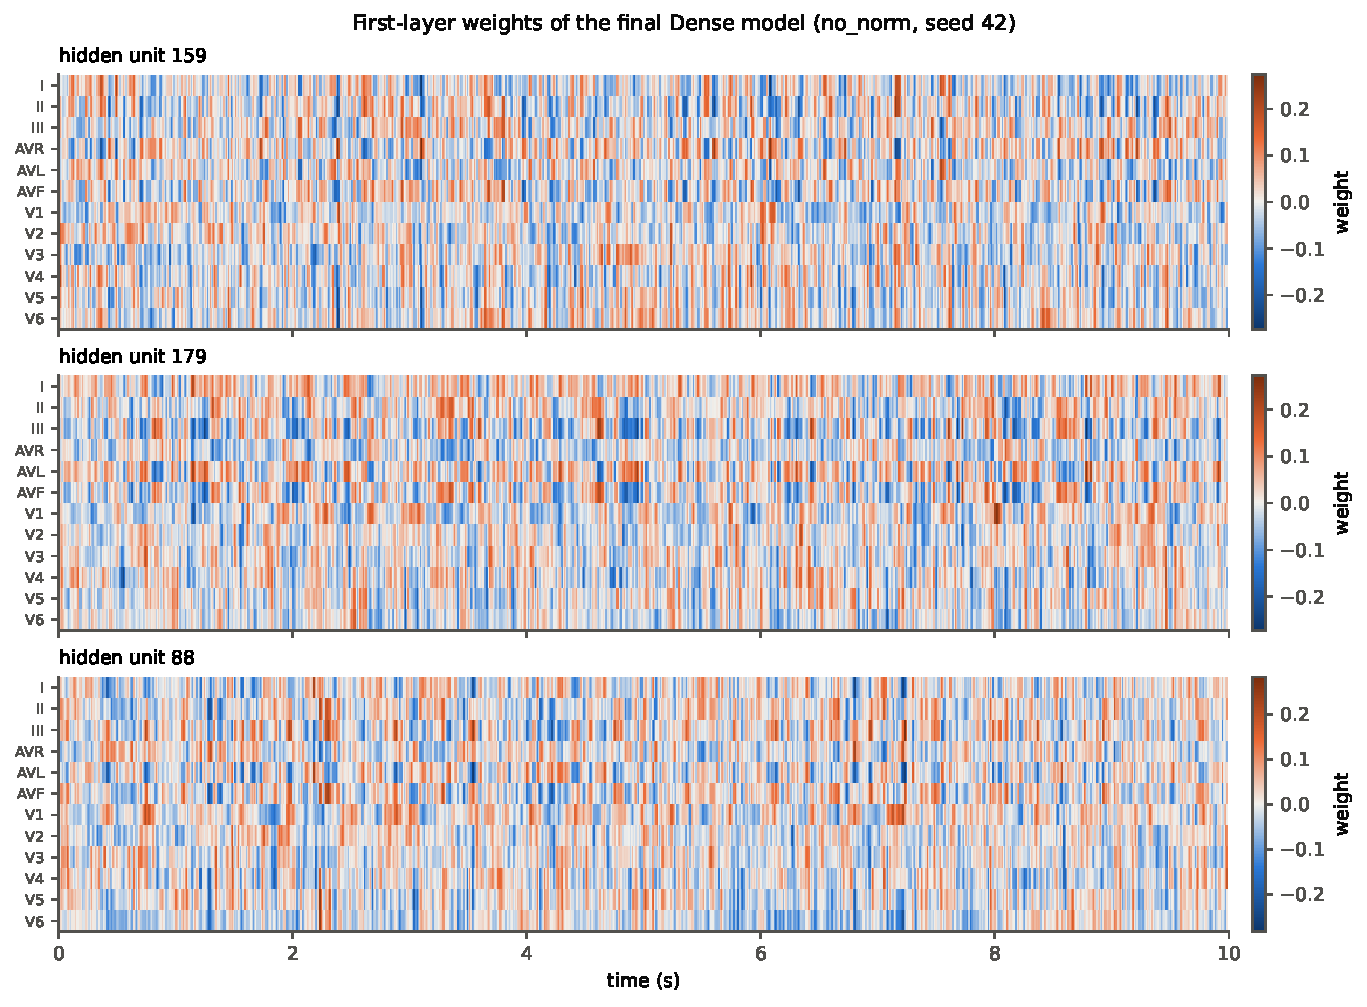
\includegraphics[width=\textwidth,height=0.42\textheight,keepaspectratio]{figures/dense_first_layer.pdf}
\caption[Dense network: first-layer weights]{First-layer weights of the final Dense model (\texttt{no\_norm}, seed 42) for the three hidden units with the largest weight norm, reshaped to 12 leads $\times$ 1000 samples.}
\label{fig:dense_first_layer}
\end{figure}


\paragraph{Selection caveat.} The rule fixed before the runs selected \texttt{no\_norm}
(no input z-score), whose validation AUROC is above the baseline's but whose paired interval contains
0 in every seed. It is the baseline without input standardisation, statistically indistinguishable
from it.

% ---------------------------------------------------------------------
\subsection{1D convolutional network (own block)}\label{sec:cnn}

\paragraph{Model and theory.} A 1D convolution slides a small filter along time: a first-layer
filter has $12\times7$ weights (all leads, seven samples, i.e.\ 70\,ms at 100\,Hz) and the same weights
are applied at every position. This \emph{weight sharing} makes the response to a QRS complex the same
wherever it occurs (translation equivariance) and divides the number of parameters by the length of
the signal. The baseline stacks four residual blocks (Conv--BN--ReLU--Conv--BN, the shortcut added,
ReLU, max pooling by 2) with 32, 64, 128 and 128 channels, followed by \emph{global average pooling}
over time, dropout and a Linear layer (\cnnParamsBase{} parameters, fewer than the Dense network).
Global average pooling turns each final feature map into one number, so the classifier sees how much
of each learnt pattern the record contains, not where. One position of the last feature map depends
on \cnnRfSamplesBase{} input samples (its \emph{receptive field}, about two seconds).

The block structure follows the residual building block of He et al., with a ``projection shortcut
\ldots\ done by 1$\times$1 convolutions'' where the number of channels changes
\cite[p.~4]{he2016deep}; batch norm and the 1D ``same'' padding are our adaptation. A residual block
learns $F(x)$ and outputs $F(x)+x$: if the identity is the best mapping, it only has to push $F$ to
zero, and the gradient flows unchanged through the addition. He et al.\ motivate it by the degradation
of plain networks: ``the deeper 34-layer plain net has higher validation error than the shallower
18-layer plain net'' \cite[p.~4]{he2016deep}. Our CNNs have at most twelve convolutional layers.

\paragraph{Results.} The CNN changes the picture completely (Tables~\ref{tab:cnn_ablations}
and~\ref{tab:cnn_final}).

% Shared float (common/make_floats.py). Table: tables/cnn_ablations.tex
\begin{table}[htbp]
\centering
\caption[1D CNN: ablations (validation)]{CNN ablations on the validation fold (same conventions as Table~\ref{tab:dense_ablations}). RF: receptive field of one position of the last feature map, in input samples.}
\label{tab:cnn_ablations}
\small
\begin{adjustbox}{max width=\textwidth}
% Generated by src/cnn_experiments.py from results/logs/cnn_summary.json.
% Needs report/numbers.tex (alias "cnn" in report/runs.json) and \usepackage{booktabs}.
% Delta: paired difference with the reference trained with the same seed (the baseline unless the label says otherwise).
\begin{tabular}{llrrcrc}
\toprule
Factor & Configuration & Parameters & RF (samples) & Val.\ macro AUROC & $\Delta$ vs.\ reference & Seeds better / worse \\
\midrule
baseline & Baseline: 4 residual blocks, kernel 7, BN, GAP, dropout 0.5 & \cnnParamsBase{} & \cnnRfSamplesBase{} & \cnnValAurocMeanBase{} $\pm$ \cnnValAurocSdBase{} & --- & --- \\
\addlinespace
kernel size & Kernel 3 & \cnnParamsKernelThree{} & \cnnRfSamplesKernelThree{} & \cnnValAurocMeanKernelThree{} $\pm$ \cnnValAurocSdKernelThree{} & \cnnDiffMeanKernelThree{} & \cnnNSeedsBetterKernelThree{} / \cnnNSeedsWorseKernelThree{} of \cnnNSeedsComparedKernelThree{} \\
kernel size & Kernel 15 & \cnnParamsKernelOneFive{} & \cnnRfSamplesKernelOneFive{} & \cnnValAurocMeanKernelOneFive{} $\pm$ \cnnValAurocSdKernelOneFive{} & \cnnDiffMeanKernelOneFive{} & \cnnNSeedsBetterKernelOneFive{} / \cnnNSeedsWorseKernelOneFive{} of \cnnNSeedsComparedKernelOneFive{} \\
\addlinespace
number of blocks & 2 blocks & \cnnParamsDepthTwo{} & \cnnRfSamplesDepthTwo{} & \cnnValAurocMeanDepthTwo{} $\pm$ \cnnValAurocSdDepthTwo{} & \cnnDiffMeanDepthTwo{} & \cnnNSeedsBetterDepthTwo{} / \cnnNSeedsWorseDepthTwo{} of \cnnNSeedsComparedDepthTwo{} \\
number of blocks & 6 blocks & \cnnParamsDepthSix{} & \cnnRfSamplesDepthSix{} & \cnnValAurocMeanDepthSix{} $\pm$ \cnnValAurocSdDepthSix{} & \cnnDiffMeanDepthSix{} & \cnnNSeedsBetterDepthSix{} / \cnnNSeedsWorseDepthSix{} of \cnnNSeedsComparedDepthSix{} \\
\addlinespace
batch norm & No batch norm & \cnnParamsNoBn{} & \cnnRfSamplesNoBn{} & \cnnValAurocMeanNoBn{} $\pm$ \cnnValAurocSdNoBn{} & \cnnDiffMeanNoBn{} & \cnnNSeedsBetterNoBn{} / \cnnNSeedsWorseNoBn{} of \cnnNSeedsComparedNoBn{} \\
\addlinespace
residual connections & No residual connections & \cnnParamsNoResidual{} & \cnnRfSamplesNoResidual{} & \cnnValAurocMeanNoResidual{} $\pm$ \cnnValAurocSdNoResidual{} & \cnnDiffMeanNoResidual{} & \cnnNSeedsBetterNoResidual{} / \cnnNSeedsWorseNoResidual{} of \cnnNSeedsComparedNoResidual{} \\
\addlinespace
residual connections $\times$ depth & 6 blocks, no residual (vs. 6 blocks) & \cnnParamsDepthSixNoResidual{} & \cnnRfSamplesDepthSixNoResidual{} & \cnnValAurocMeanDepthSixNoResidual{} $\pm$ \cnnValAurocSdDepthSixNoResidual{} & \cnnDiffMeanDepthSixNoResidual{} & \cnnNSeedsBetterDepthSixNoResidual{} / \cnnNSeedsWorseDepthSixNoResidual{} of \cnnNSeedsComparedDepthSixNoResidual{} \\
\addlinespace
global pooling vs flatten & Flatten instead of global average pooling & \cnnParamsFlatten{} & \cnnRfSamplesFlatten{} & \cnnValAurocMeanFlatten{} $\pm$ \cnnValAurocSdFlatten{} & \cnnDiffMeanFlatten{} & \cnnNSeedsBetterFlatten{} / \cnnNSeedsWorseFlatten{} of \cnnNSeedsComparedFlatten{} \\
\addlinespace
dropout & No dropout & \cnnParamsNoDropout{} & \cnnRfSamplesNoDropout{} & \cnnValAurocMeanNoDropout{} $\pm$ \cnnValAurocSdNoDropout{} & \cnnDiffMeanNoDropout{} & \cnnNSeedsBetterNoDropout{} / \cnnNSeedsWorseNoDropout{} of \cnnNSeedsComparedNoDropout{} \\
\bottomrule
\end{tabular}

\end{adjustbox}
\end{table}

% Shared float (common/make_floats.py). Table: tables/cnn_final.tex
\begin{table}[htbp]
\centering
\caption[1D CNN: final model (test)]{Final CNN (\texttt{no\_dropout}) on the test fold, with the final Dense and trivial models, and paired differences per seed (95\,\% patient bootstrap).}
\label{tab:cnn_final}
\small
\begin{adjustbox}{max width=\textwidth}
% Generated by src/cnn_experiments.py from results/logs/cnn_summary.json.
% Needs report/numbers.tex (aliases "cnn", "trivial" and "dense").
\begin{tabular}{lcccc}
\toprule
 & \multicolumn{2}{c}{CNN (final)} & Dense (final) & Trivial \\
\cmidrule(lr){2-3}
Test AUROC & First seed [95\% CI] & Mean $\pm$ SD (seeds) & Mean $\pm$ SD &  \\
\midrule
Macro & \cnnFinalFirstTestMacroAuroc{} [\cnnFinalFirstTestMacroAurocLo{}, \cnnFinalFirstTestMacroAurocHi{}] & \cnnFinalTestMacroAurocMean{} $\pm$ \cnnFinalTestMacroAurocSd{} & \denseFinalTestMacroAurocMean{} $\pm$ \denseFinalTestMacroAurocSd{} & \trivialTestMacroAuroc{} \\
\midrule
NORM & \cnnFinalFirstTestAurocNORM{} [\cnnFinalFirstTestAurocNORMLo{}, \cnnFinalFirstTestAurocNORMHi{}] & \cnnFinalTestAurocNORMMean{} $\pm$ \cnnFinalTestAurocNORMSd{} & \denseFinalTestAurocNORMMean{} $\pm$ \denseFinalTestAurocNORMSd{} & \trivialTestAurocNORM{} \\
MI & \cnnFinalFirstTestAurocMI{} [\cnnFinalFirstTestAurocMILo{}, \cnnFinalFirstTestAurocMIHi{}] & \cnnFinalTestAurocMIMean{} $\pm$ \cnnFinalTestAurocMISd{} & \denseFinalTestAurocMIMean{} $\pm$ \denseFinalTestAurocMISd{} & \trivialTestAurocMI{} \\
STTC & \cnnFinalFirstTestAurocSTTC{} [\cnnFinalFirstTestAurocSTTCLo{}, \cnnFinalFirstTestAurocSTTCHi{}] & \cnnFinalTestAurocSTTCMean{} $\pm$ \cnnFinalTestAurocSTTCSd{} & \denseFinalTestAurocSTTCMean{} $\pm$ \denseFinalTestAurocSTTCSd{} & \trivialTestAurocSTTC{} \\
CD & \cnnFinalFirstTestAurocCD{} [\cnnFinalFirstTestAurocCDLo{}, \cnnFinalFirstTestAurocCDHi{}] & \cnnFinalTestAurocCDMean{} $\pm$ \cnnFinalTestAurocCDSd{} & \denseFinalTestAurocCDMean{} $\pm$ \denseFinalTestAurocCDSd{} & \trivialTestAurocCD{} \\
HYP & \cnnFinalFirstTestAurocHYP{} [\cnnFinalFirstTestAurocHYPLo{}, \cnnFinalFirstTestAurocHYPHi{}] & \cnnFinalTestAurocHYPMean{} $\pm$ \cnnFinalTestAurocHYPSd{} & \denseFinalTestAurocHYPMean{} $\pm$ \denseFinalTestAurocHYPSd{} & \trivialTestAurocHYP{} \\
\midrule
$\Delta$ macro vs.\ Dense, seed 42 & \cnnDiffDenseSFourTwo{} [\cnnDiffDenseLoSFourTwo{}, \cnnDiffDenseHiSFourTwo{}] & & & \\
$\Delta$ macro vs.\ Dense, seed 43 & \cnnDiffDenseSFourThree{} [\cnnDiffDenseLoSFourThree{}, \cnnDiffDenseHiSFourThree{}] & & & \\
$\Delta$ macro vs.\ Dense, seed 44 & \cnnDiffDenseSFourFour{} [\cnnDiffDenseLoSFourFour{}, \cnnDiffDenseHiSFourFour{}] & & & \\
$\Delta$ macro vs.\ trivial, seed 42 & \cnnDiffTrivialSFourTwo{} [\cnnDiffTrivialLoSFourTwo{}, \cnnDiffTrivialHiSFourTwo{}] & & & \\
$\Delta$ macro vs.\ trivial, seed 43 & \cnnDiffTrivialSFourThree{} [\cnnDiffTrivialLoSFourThree{}, \cnnDiffTrivialHiSFourThree{}] & & & \\
$\Delta$ macro vs.\ trivial, seed 44 & \cnnDiffTrivialSFourFour{} [\cnnDiffTrivialLoSFourFour{}, \cnnDiffTrivialHiSFourFour{}] & & & \\
\bottomrule
\end{tabular}

\end{adjustbox}
\end{table}

% Shared float (common/make_floats.py). Figure: figures/cnn_curves.pdf
\begin{figure}[htbp]
\centering
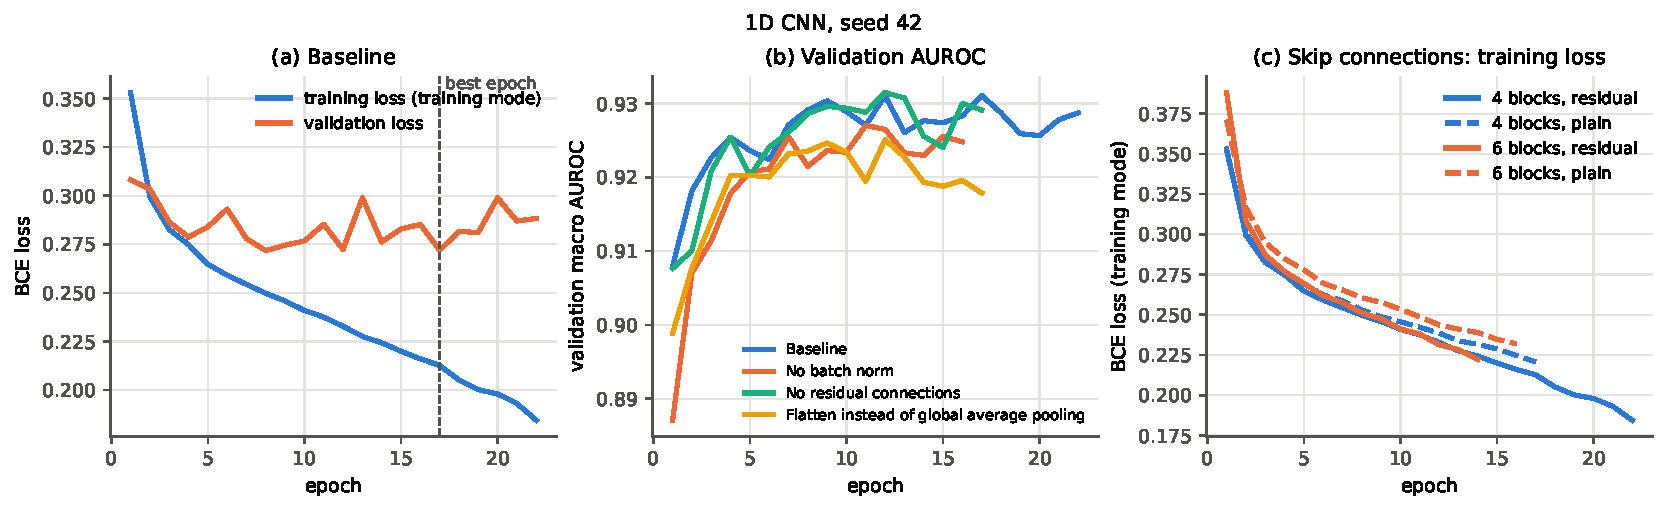
\includegraphics[width=\textwidth,height=0.42\textheight,keepaspectratio]{figures/cnn_curves.pdf}
\caption[1D CNN: learning curves]{1D CNN, seed 42. (a) Baseline training and validation loss; dashed line: best epoch. (b) Validation macro AUROC without batch norm, without residual connections and with flatten instead of global average pooling. (c) Training loss with and without residual connections, at 4 and 6 blocks.}
\label{fig:cnn_curves}
\end{figure}


\begin{enumerate}[leftmargin=1.4em,itemsep=2pt]
  \item \textbf{Convolutions are the change that matters.} The final CNN gains \cnnDiffDenseMean{}
        of test macro AUROC over the final Dense network, in every seed and in every class, with far
        fewer parameters. The largest effect of any Dense ablation was several times smaller.
  \item \textbf{Inside the CNN, no factor matters much.} The ten configurations lie between
        \cnnValAurocMeanFlatten{} and \cnnValAurocMeanNoDropout{} on validation
        (Table~\ref{tab:cnn_ablations}). The network is robust to these choices, and differences of
        a few thousandths should not be over-interpreted. Only flatten (\cnnDiffMeanFlatten{}) and no
        batch norm (\cnnDiffMeanNoBn{}) are worse in two seeds of three.
  \item \textbf{Global pooling against flatten.} Flatten gives the classifier one weight per channel
        and position, so it loses the translation invariance of the head; it is slightly worse and fits
        the training set faster (training loss at epoch 5 \cnnTrainLossEpFiveDiffMeanFlatten{} with
        respect to the baseline). It is the Dense network's problem on a small scale.
  \item \textbf{Batch norm matters much less than in the Dense network} (\cnnDiffMeanNoBn{} here,
        \denseDiffMeanNoBn{} there). Without it the CNN learns more slowly (best epoch
        \intval{\cnnBestEpochMeanNoBn} against \intval{\cnnBestEpochMeanBase}) but reaches almost the
        same result. My explanation, not tested: the convolutions see small windows of an already
        standardised input and have few parameters.
  \item \textbf{Skip connections: no measurable effect at this depth.} The validation AUROC does not
        change without them (\cnnDiffMeanNoResidual{} with four blocks, \cnnDiffMeanDepthSixNoResidual{}
        with six). Without them the training loss at epoch 5 is slightly higher
        (\cnnTrainLossEpFiveDiffMeanNoResidual{} with four blocks, \cnnTrainLossEpFiveDiffMeanDepthSixNoResidual{}
        with six; Figure~\ref{fig:cnn_curves}c), which points in the direction of the degradation argument,
        but this is weak evidence: almost every change of the baseline (kernel size, depth, batch norm)
        also raises that loss in all seeds, and the loss is a single number without an interval. With at
        most twelve layers and early stopping after about ten epochs, our networks are far shallower than
        those in which He et al.\ observed degradation.
  \item \textbf{A wide range of receptive fields gives the same result.} Receptive fields from
        \cnnRfSamplesDepthTwo{} to \cnnRfSamplesDepthSix{} samples (two blocks to six) all reach the
        same level; even two blocks, whose receptive field is shorter than one beat, match the
        baseline, although they fit the training set more slowly. For these five superclasses, local
        beat-level patterns averaged over the record seem to be enough (an interpretation, not a
        tested claim).
  \item \textbf{Dropout before the classifier does not help} (no dropout: \cnnDiffMeanNoDropout{}).
        After global average pooling the classifier has only a few hundred parameters, so there is
        little to regularise, unlike the Dense network.
\end{enumerate}

\paragraph{What the CNN learnt.} The first-layer filters do not look like heartbeat templates, but
their frequency responses form a bank of mostly low-frequency filters (Figure~\ref{fig:cnn_first_layer}):
median peak \onedec{\cnnFirstLayerPeakHzMedian}\,Hz, \cnnFirstLayerNPeakBelowFiveHz{} of
\cnnFirstLayerNFilters{} below 5\,Hz and \cnnFirstLayerNPeakAboveTwoZeroHz{} above 20\,Hz. This is
consistent with the main ECG waves lying below 50\,Hz (P wave 0.67--5\,Hz, T wave 1--7\,Hz, QRS
10--50\,Hz \cite[p.~12]{adam2025comparative}); the figure only shows what the network kept. In the
feature maps (Figure~\ref{fig:cnn_feature_maps}) the channels of the first block fire at every QRS
complex, the same filter applied at every position, and the last block still shows bands aligned with
the beats. The class activation map (CAM) decomposes the logit over time: with global average pooling
and one Linear layer, $z_c = b_c + \frac{1}{T}\sum_t \mathrm{CAM}_c(t)$. The idea is from Zhou et al.,
who ``ignore the bias term'' \cite[pp.~2--3]{zhou2016learning}; our variant keeps it and uses the mean.
The map must be read together with the prediction: the MI, CD and HYP examples are classified
correctly, the NORM and STTC examples are missed, and the STTC map is negative almost throughout. A
CAM shows where the evidence for or against a class lies, also when the model is wrong.

% Shared float (common/make_floats.py). Figure: figures/cnn_first_layer.pdf
\begin{figure}[htbp]
\centering
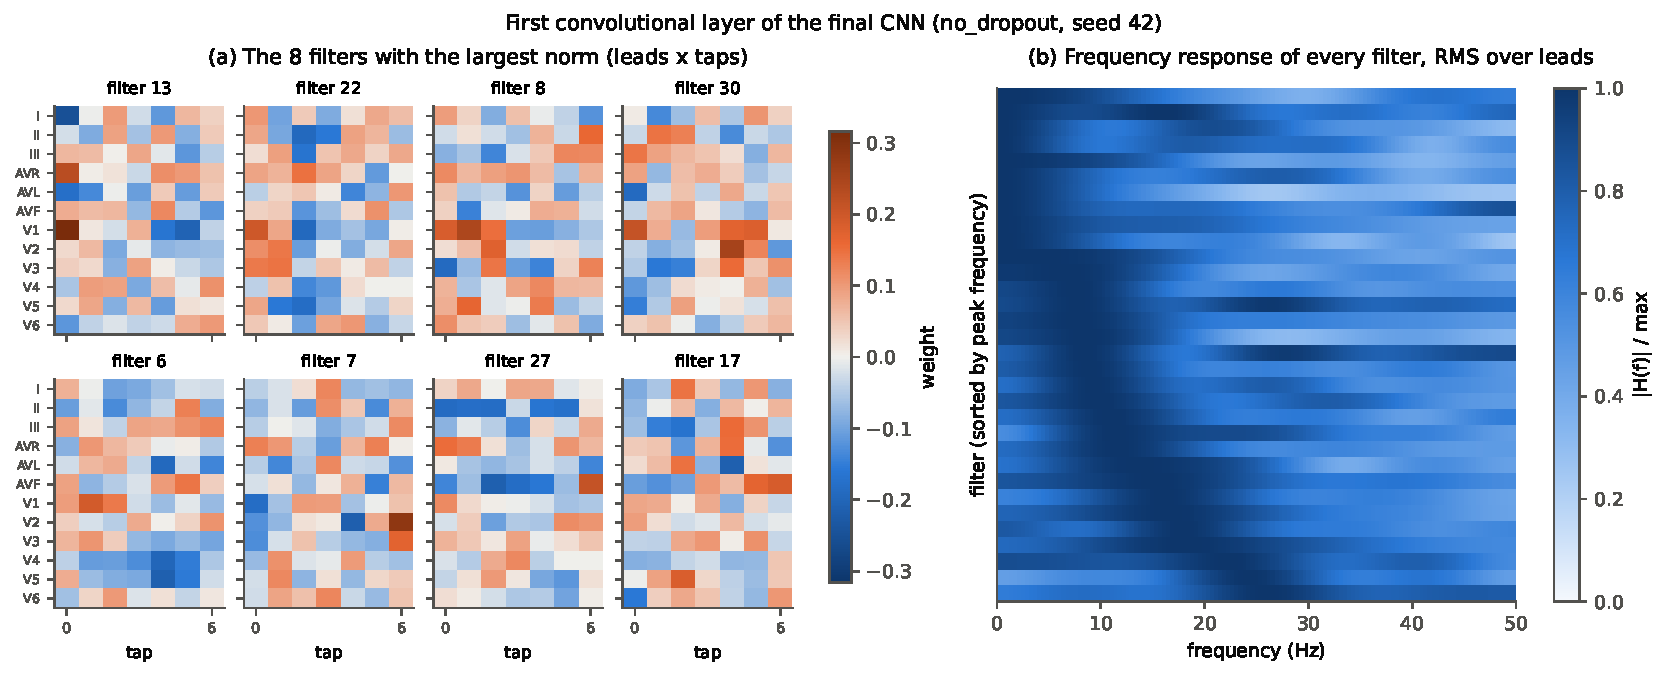
\includegraphics[width=\textwidth,height=0.42\textheight,keepaspectratio]{figures/cnn_first_layer.pdf}
\caption[1D CNN: first-layer filters]{First convolutional layer of the final CNN (\texttt{no\_dropout}, seed 42). (a) The eight filters with the largest norm (12 leads $\times$ 7 taps). (b) Frequency response of every filter (RMS over leads, normalised), sorted by peak frequency.}
\label{fig:cnn_first_layer}
\end{figure}

% Shared float (common/make_floats.py). Figure: figures/cnn_feature_maps.pdf
\begin{figure}[htbp]
\centering
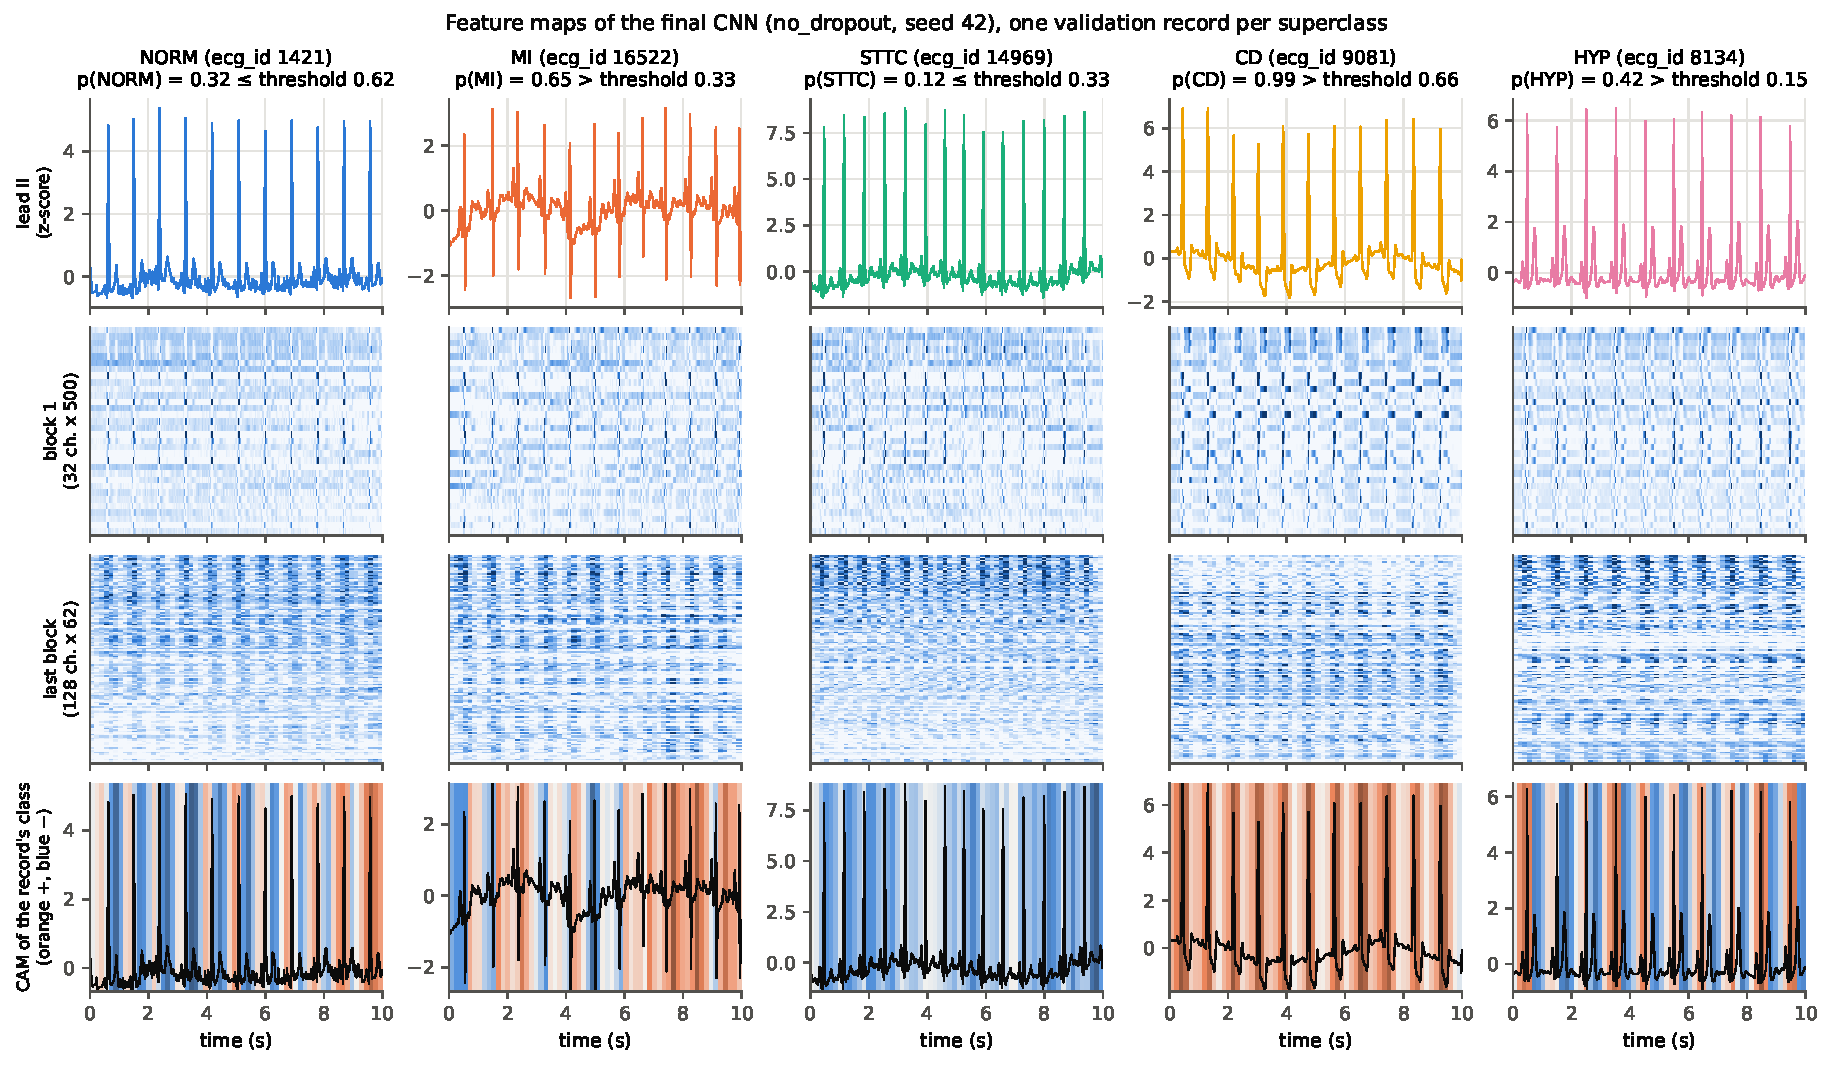
\includegraphics[width=\textwidth,height=0.42\textheight,keepaspectratio]{figures/cnn_feature_maps.pdf}
\caption[1D CNN: feature maps and class activation maps]{Final CNN on one validation record per superclass (seed 42). Rows: lead II (z-score), feature maps of block 1 and of the last block, and the class activation map of the record's class (orange: evidence for the class, blue: against). Column titles: predicted probability and the class threshold chosen on validation; NORM and STTC are missed.}
\label{fig:cnn_feature_maps}
\end{figure}


\paragraph{Selection caveat.} The rule selected \texttt{no\_dropout}, better than the baseline in one
seed of three only: the final CNN is the baseline without dropout, statistically close to it.

% ---------------------------------------------------------------------
\subsection{Recurrent networks and RNN + attention (Mar\'ia's block, summary)}\label{sec:rnn}

\paragraph{Theory.} A recurrent network reads the sequence step by step and updates a hidden state
$h_t = f(h_{t-1}, x_t)$ with the same weights at every step, so it also shares weights over time.
Gradients through many steps tend to vanish or explode; the LSTM and the GRU control them with gates
that decide what to keep, write and output. The GRU was ``motivated by the LSTM unit but is much
simpler to compute and implement'' \cite[p.~1725]{cho2014learning}, and a large comparison of LSTM
variants found that ``none of the variants can improve upon the standard LSTM architecture
significantly'' \cite[p.~1]{greff2017lstm}. Exploding gradients were handled with gradient clipping,
which ``has been shown to do well in practice'' \cite[p.~6]{pascanu2013difficulty}. With attention,
instead of using only the last state, a score is computed for every state, a softmax over time turns
the scores into weights $\alpha_t$, and the classifier sees $\sum_t \alpha_t h_t$; the score function is
an ``alignment model'' in the sense of Bahdanau et al.\ \cite[p.~3]{bahdanau2015neural}.

\paragraph{Results (Mar\'ia).} The baseline is a two-layer LSTM over 100 frames of 100\,ms. The GRU
was better than the LSTM (\rnnDiffMeanGru{}, all seeds); using every state (mean
\rnnDiffMeanMean{}, attention \rnnDiffMeanAttn{}) mattered more than the direction;
1000 raw steps beat 100 frames (\rnnDiffMeanRaw{}) although they were much harder to optimise; and a
convolutional front end was the best configuration (\rnnDiffMeanConv{}), which became the final RNN.
Its test macro AUROC is \rnnFinalTestMacroAurocMean{}, below the CNN in every seed
(\rnnDiffCnnMean{}). In the five example records of Figure~\ref{fig:rnn_attention} the attention weights seem to rise and
fall with the heartbeat, but this is a visual observation that the correlation measured by Mar\'ia does
not confirm (\rnnAttnSpearmanActivityRawAttn{}); what is measured is that the weights are spread out (for additive attention over 100 frames, normalised
entropy \rnnAttnEntropyNormAttn{}, where 1 is uniform): in this task attention behaves like a learned mean and gains as much as plain
averaging. The final RNN + attention (\rnnAttnfinalTestMacroAurocMean{} on test) cannot be told apart
from the final RNN. My reading of the two blocks together: what helps is weight sharing over time,
which the CNN provides most directly.

% Shared float (common/make_floats.py). Figure: figures/rnn_attention.pdf
\begin{figure}[htbp]
\centering
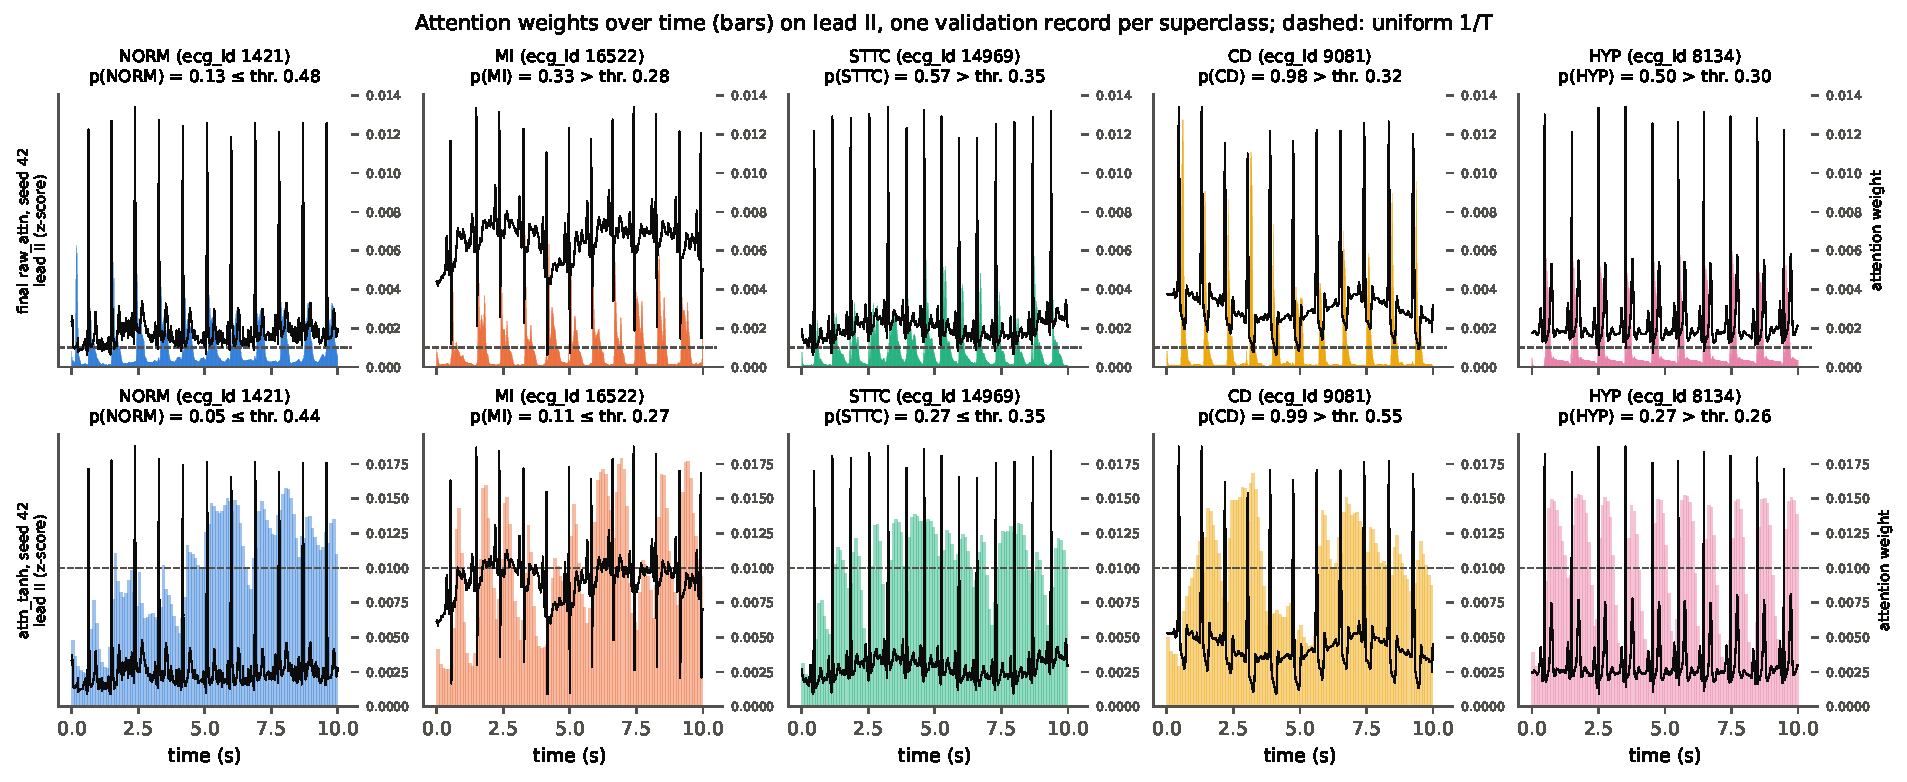
\includegraphics[width=\textwidth,height=0.42\textheight,keepaspectratio]{figures/rnn_attention.pdf}
\caption[RNN + attention: attention weights over time]{Attention weights over time (bars) on lead II for one validation record per superclass: final RNN + attention (\texttt{raw\_attn}, top) and the notebook tanh score over 100 frames (bottom); dashed: uniform weight $1/T$. Titles: predicted probability and threshold.}
\label{fig:rnn_attention}
\end{figure}


% ---------------------------------------------------------------------
\subsection{Self-attention and the Transformer (Mar\'ia's block, summary)}\label{sec:transformer}

\paragraph{Theory.} Self-attention lets every token build its output from all the others: queries,
keys and values are linear projections of the tokens, and each output is a weighted sum of the
values, with weights $\mathrm{softmax}(QK^\top/\sqrt{d_k})$ (``Scaled Dot-Product Attention''
\cite[p.~4]{vaswani2017attention}). Several heads in parallel let the model ``jointly attend to
information from different representation subspaces at different positions''
\cite[p.~5]{vaswani2017attention}. A Transformer block adds a feed-forward network, residual
connections and layer normalisation; the original placed it after each residual addition
(``LayerNorm(x + Sublayer(x))'' \cite[p.~3]{vaswani2017attention}), and the course notes that
placing it before (Pre-LN) ``simply makes the optimization much easier''
\cite{course_transformer_part2}. Attention ignores order, so a positional encoding (sine and cosine
functions \cite[p.~6]{vaswani2017attention}) is added to the tokens.

\paragraph{Results (Mar\'ia).} The record is cut into 100 patches of 100\,ms, each projected to a
token. Built step by step (Figure~\ref{fig:transformer_curves}b), one single-head attention layer
already reaches \transformerValAurocMeanSaSingle{} on validation, far above the Dense network, which
Mar\'ia attributes to the same projection being applied to every patch; multiple heads and the residual path with LayerNorm
give the largest further gains, and the paired difference between a bare attention layer and a
full block is \transformerPairSaVsBlockMean{}, worse in all seeds. The models do not use the order
of the patches: shuffling them changes the validation AUROC by about a thousandth, and removing the
positional encoding was better (\transformerDiffMeanNoPos{}, all seeds), so the final Transformer
(\texttt{no\_pos}) classifies the \emph{set} of patches. On test it reaches
\transformerFinalTestMacroAurocMean{}, below the CNN (\transformerDiffCnnMean{}) and the RNN
(\transformerDiffRnnMean{}) in every seed.

% Shared float (common/make_floats.py). Figure: figures/transformer_curves.pdf
\begin{figure}[htbp]
\centering
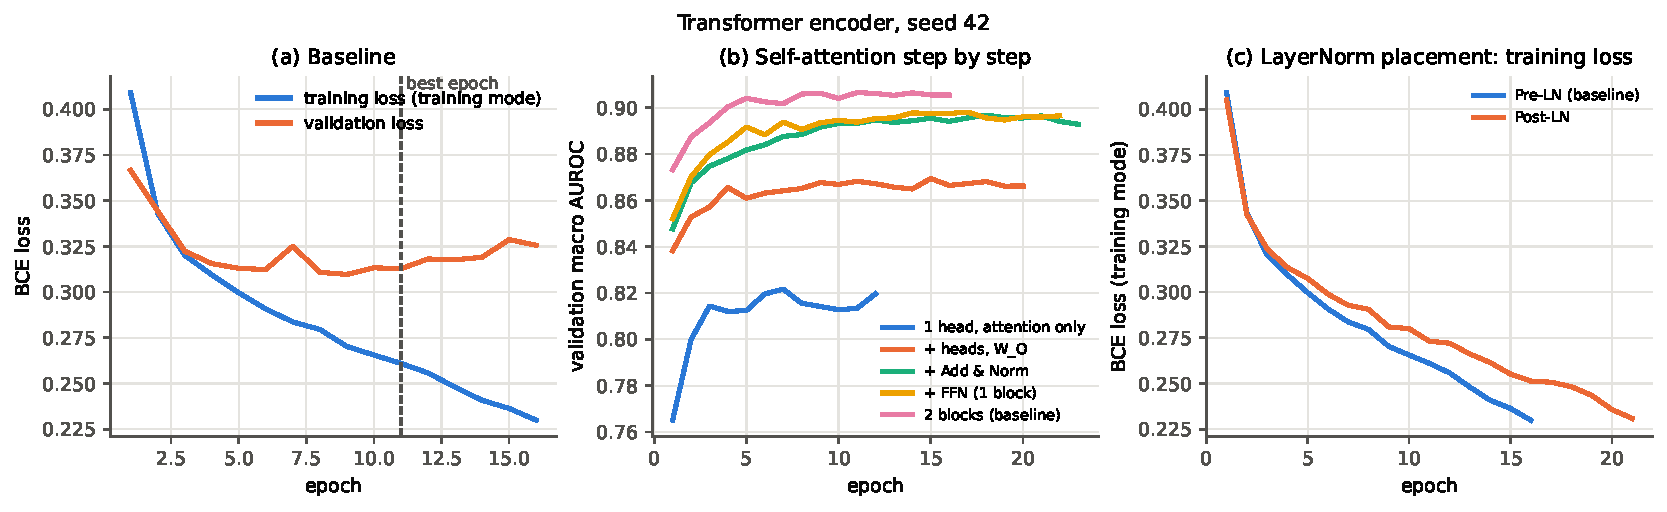
\includegraphics[width=\textwidth,height=0.42\textheight,keepaspectratio]{figures/transformer_curves.pdf}
\caption[Transformer: learning curves and self-attention step by step]{Transformer encoder, seed 42. (a) Baseline losses. (b) Self-attention step by step: validation macro AUROC from one single-head attention layer to two full blocks. (c) Training loss with Pre-LN and Post-LN.}
\label{fig:transformer_curves}
\end{figure}


% ---------------------------------------------------------------------
\subsection{Across families: twelve leads against lead II}\label{sec:leads}

The final model of each family was trained again on lead II only (shared task T14,
Table~\ref{tab:leads}). Every family loses in every seed, by a similar amount, and the CNN stays first.
The other eleven leads are not redundant with lead II for these superclasses; MI and HYP lose most
(Table~\ref{tab:comparison_per_class}). For part of MI there is a reason in the literature: anterior
infarction is ``expressed as ST elevation in some or all of leads V1 through V6''
\cite[p.~e265]{wagner2009aha}, chest leads that a lead-II model never sees. This explains at most the
anterior infarctions, not every MI record; for HYP and the other classes any explanation would be a
hypothesis.

% Shared float (common/make_floats.py). Table: tables/leads.tex
\begin{table}[htbp]
\centering
\caption[12 leads against lead II]{12 leads against lead II only, final model of each family (test fold, mean over seeds; $\Delta$ = paired difference, lead II minus 12 leads).}
\label{tab:leads}
\small
\begin{adjustbox}{max width=\textwidth}
% Generated by src/leads_experiments.py from results/logs/leads_summary.json.
% Needs report/numbers.tex (alias "leads") and booktabs.
\begin{tabular}{llrccrc}
\toprule
Family & Final config. & Param.\ (12 / 1) & Test AUROC, 12 leads & Test AUROC, lead II & $\Delta$ & Seeds better / worse \\
\midrule
Dense & \texttt{no\_norm} & \leadsParamsTwelveDense{} / \leadsParamsOneleadDense{} & \leadsTestAurocMeanTwelveDense{} $\pm$ \leadsTestAurocSdTwelveDense{} & \leadsTestAurocMeanOneleadDense{} $\pm$ \leadsTestAurocSdOneleadDense{} & \leadsTestDiffMeanDense{} & \leadsTestNBetterDense{} / \leadsTestNWorseDense{} of \leadsTestNComparedDense{} \\
CNN & \texttt{no\_dropout} & \leadsParamsTwelveCnn{} / \leadsParamsOneleadCnn{} & \leadsTestAurocMeanTwelveCnn{} $\pm$ \leadsTestAurocSdTwelveCnn{} & \leadsTestAurocMeanOneleadCnn{} $\pm$ \leadsTestAurocSdOneleadCnn{} & \leadsTestDiffMeanCnn{} & \leadsTestNBetterCnn{} / \leadsTestNWorseCnn{} of \leadsTestNComparedCnn{} \\
RNN & \texttt{conv} & \leadsParamsTwelveRnn{} / \leadsParamsOneleadRnn{} & \leadsTestAurocMeanTwelveRnn{} $\pm$ \leadsTestAurocSdTwelveRnn{} & \leadsTestAurocMeanOneleadRnn{} $\pm$ \leadsTestAurocSdOneleadRnn{} & \leadsTestDiffMeanRnn{} & \leadsTestNBetterRnn{} / \leadsTestNWorseRnn{} of \leadsTestNComparedRnn{} \\
RNN + attention & \texttt{raw\_attn} & \leadsParamsTwelveRnnattn{} / \leadsParamsOneleadRnnattn{} & \leadsTestAurocMeanTwelveRnnattn{} $\pm$ \leadsTestAurocSdTwelveRnnattn{} & \leadsTestAurocMeanOneleadRnnattn{} $\pm$ \leadsTestAurocSdOneleadRnnattn{} & \leadsTestDiffMeanRnnattn{} & \leadsTestNBetterRnnattn{} / \leadsTestNWorseRnnattn{} of \leadsTestNComparedRnnattn{} \\
Transformer & \texttt{no\_pos} & \leadsParamsTwelveTransformer{} / \leadsParamsOneleadTransformer{} & \leadsTestAurocMeanTwelveTransformer{} $\pm$ \leadsTestAurocSdTwelveTransformer{} & \leadsTestAurocMeanOneleadTransformer{} $\pm$ \leadsTestAurocSdOneleadTransformer{} & \leadsTestDiffMeanTransformer{} & \leadsTestNBetterTransformer{} / \leadsTestNWorseTransformer{} of \leadsTestNComparedTransformer{} \\
\bottomrule
\end{tabular}

\end{adjustbox}
\end{table}

% Shared float (common/make_floats.py). Table: tables/comparison_per_class.tex
\begin{table}[htbp]
\centering
\caption[Test AUROC per superclass]{Test AUROC per superclass of every final model (mean over seeds).}
\label{tab:comparison_per_class}
\small
\begin{adjustbox}{max width=\textwidth}
% Generated by src/comparison.py: test AUROC per superclass, mean over seeds.
\begin{tabular}{lccccc}
\toprule
Model & NORM & MI & STTC & CD & HYP \\
\midrule
\multicolumn{6}{l}{\textit{12 leads}} \\
\quad Trivial (lead mean and SD) & \comparisonTestAurocNORMMeanTrivial{} & \comparisonTestAurocMIMeanTrivial{} & \comparisonTestAurocSTTCMeanTrivial{} & \comparisonTestAurocCDMeanTrivial{} & \comparisonTestAurocHYPMeanTrivial{} \\
\quad Dense & \comparisonTestAurocNORMMeanTwelveDense{} & \comparisonTestAurocMIMeanTwelveDense{} & \comparisonTestAurocSTTCMeanTwelveDense{} & \comparisonTestAurocCDMeanTwelveDense{} & \comparisonTestAurocHYPMeanTwelveDense{} \\
\quad CNN & \comparisonTestAurocNORMMeanTwelveCnn{} & \comparisonTestAurocMIMeanTwelveCnn{} & \comparisonTestAurocSTTCMeanTwelveCnn{} & \comparisonTestAurocCDMeanTwelveCnn{} & \comparisonTestAurocHYPMeanTwelveCnn{} \\
\quad RNN & \comparisonTestAurocNORMMeanTwelveRnn{} & \comparisonTestAurocMIMeanTwelveRnn{} & \comparisonTestAurocSTTCMeanTwelveRnn{} & \comparisonTestAurocCDMeanTwelveRnn{} & \comparisonTestAurocHYPMeanTwelveRnn{} \\
\quad RNN + attention & \comparisonTestAurocNORMMeanTwelveRnnattn{} & \comparisonTestAurocMIMeanTwelveRnnattn{} & \comparisonTestAurocSTTCMeanTwelveRnnattn{} & \comparisonTestAurocCDMeanTwelveRnnattn{} & \comparisonTestAurocHYPMeanTwelveRnnattn{} \\
\quad Transformer & \comparisonTestAurocNORMMeanTwelveTransformer{} & \comparisonTestAurocMIMeanTwelveTransformer{} & \comparisonTestAurocSTTCMeanTwelveTransformer{} & \comparisonTestAurocCDMeanTwelveTransformer{} & \comparisonTestAurocHYPMeanTwelveTransformer{} \\
\multicolumn{6}{l}{\textit{Lead II only (T14)}} \\
\quad Dense & \comparisonTestAurocNORMMeanOneleadDense{} & \comparisonTestAurocMIMeanOneleadDense{} & \comparisonTestAurocSTTCMeanOneleadDense{} & \comparisonTestAurocCDMeanOneleadDense{} & \comparisonTestAurocHYPMeanOneleadDense{} \\
\quad CNN & \comparisonTestAurocNORMMeanOneleadCnn{} & \comparisonTestAurocMIMeanOneleadCnn{} & \comparisonTestAurocSTTCMeanOneleadCnn{} & \comparisonTestAurocCDMeanOneleadCnn{} & \comparisonTestAurocHYPMeanOneleadCnn{} \\
\quad RNN & \comparisonTestAurocNORMMeanOneleadRnn{} & \comparisonTestAurocMIMeanOneleadRnn{} & \comparisonTestAurocSTTCMeanOneleadRnn{} & \comparisonTestAurocCDMeanOneleadRnn{} & \comparisonTestAurocHYPMeanOneleadRnn{} \\
\quad RNN + attention & \comparisonTestAurocNORMMeanOneleadRnnattn{} & \comparisonTestAurocMIMeanOneleadRnnattn{} & \comparisonTestAurocSTTCMeanOneleadRnnattn{} & \comparisonTestAurocCDMeanOneleadRnnattn{} & \comparisonTestAurocHYPMeanOneleadRnnattn{} \\
\quad Transformer & \comparisonTestAurocNORMMeanOneleadTransformer{} & \comparisonTestAurocMIMeanOneleadTransformer{} & \comparisonTestAurocSTTCMeanOneleadTransformer{} & \comparisonTestAurocCDMeanOneleadTransformer{} & \comparisonTestAurocHYPMeanOneleadTransformer{} \\
\multicolumn{6}{l}{\textit{Lead II, ECG-GPT transfer (T13)}} \\
\quad ECG-GPT, from scratch, 100\% & \comparisonTestAurocNORMMeanScratchFOneZeroZero{} & \comparisonTestAurocMIMeanScratchFOneZeroZero{} & \comparisonTestAurocSTTCMeanScratchFOneZeroZero{} & \comparisonTestAurocCDMeanScratchFOneZeroZero{} & \comparisonTestAurocHYPMeanScratchFOneZeroZero{} \\
\quad ECG-GPT, linear probe (frozen), 100\% & \comparisonTestAurocNORMMeanProbeFOneZeroZero{} & \comparisonTestAurocMIMeanProbeFOneZeroZero{} & \comparisonTestAurocSTTCMeanProbeFOneZeroZero{} & \comparisonTestAurocCDMeanProbeFOneZeroZero{} & \comparisonTestAurocHYPMeanProbeFOneZeroZero{} \\
\quad ECG-GPT, fine-tuning, 100\% & \comparisonTestAurocNORMMeanFinetuneFOneZeroZero{} & \comparisonTestAurocMIMeanFinetuneFOneZeroZero{} & \comparisonTestAurocSTTCMeanFinetuneFOneZeroZero{} & \comparisonTestAurocCDMeanFinetuneFOneZeroZero{} & \comparisonTestAurocHYPMeanFinetuneFOneZeroZero{} \\
\quad ECG-GPT, from scratch, 10\% & \comparisonTestAurocNORMMeanScratchFOneZero{} & \comparisonTestAurocMIMeanScratchFOneZero{} & \comparisonTestAurocSTTCMeanScratchFOneZero{} & \comparisonTestAurocCDMeanScratchFOneZero{} & \comparisonTestAurocHYPMeanScratchFOneZero{} \\
\quad ECG-GPT, linear probe (frozen), 10\% & \comparisonTestAurocNORMMeanProbeFOneZero{} & \comparisonTestAurocMIMeanProbeFOneZero{} & \comparisonTestAurocSTTCMeanProbeFOneZero{} & \comparisonTestAurocCDMeanProbeFOneZero{} & \comparisonTestAurocHYPMeanProbeFOneZero{} \\
\quad ECG-GPT, fine-tuning, 10\% & \comparisonTestAurocNORMMeanFinetuneFOneZero{} & \comparisonTestAurocMIMeanFinetuneFOneZero{} & \comparisonTestAurocSTTCMeanFinetuneFOneZero{} & \comparisonTestAurocCDMeanFinetuneFOneZero{} & \comparisonTestAurocHYPMeanFinetuneFOneZero{} \\
\multicolumn{6}{l}{\textit{Lead II, zero-shot (T24)}} \\
\quad CLIP ViT-B/32, zero-shot & \comparisonTestAurocNORMMeanZeroshot{} & \comparisonTestAurocMIMeanZeroshot{} & \comparisonTestAurocSTTCMeanZeroshot{} & \comparisonTestAurocCDMeanZeroshot{} & \comparisonTestAurocHYPMeanZeroshot{} \\
\bottomrule
\end{tabular}

\end{adjustbox}
\end{table}


\paragraph{Critical reading of area 1.} With 12 leads and with lead II alone, the CNN is first and,
among the four weight-sharing families, the Transformer last; the RNN and the RNN + attention swap
places. The gaps among these four are small compared with the gap to the Dense network. The common factor of the good models is not
recurrence or attention but sharing weights over time; the CNN encodes it most directly. The Transformer's indifference to patch order and the RNN's attention that
acts as an average both suggest that, for these superclasses, \emph{what} patterns a record contains
matters more than \emph{when} they occur, which favours a convolutional bias with global pooling. A
label set that depends on rhythm (intervals between beats) would be the test of this interpretation;
we did not run it.
